\chapter{Clustering}

In the field of clustering analysis, there is no strict definition for cluster itself. That may be one reason why there is such a vast amount of clustering algorithms; many authors such as \citet{estivill2002so} discuss this topic.  However, the one think in common that we can find among all the algorithms is a work with a group of data objects.

Suppose data $\mathcal{D}$ given as a $n$ $d$-dimensional vectors $(x_1,\dots,x_d) \subset \R_d$  -- objects; each element of a vector describes specific object property. Two objects are similar if values of their respective properties are alike. Then, clustering analysis can be defined as a form of grouping objects into subsets of $\mathbf{D}$ while maximizing inter-set object similarity and minimizing intra-set object similarity.

\section{Clustering models}

Concrete variations of clustering analysis are defined by a clustering model. They are divided into several sections.

\subsection{Centroid-based model}

\emph{Centroid-based clustering model} represents clusters only by a central vector --- \emph{centroid} --- which is not necessarily a member of a working set. Many implementations of this model need the number of required centroids in advance. We define the following optimalization problem for this kinds of algorithms. 

\begin{problem}
	Having a distance function $d$, find $k$ centroids $C_1,\dots,C_k$ from the domain of the dataset $\mathcal{D}$ such that the sum \ref{eq01:sum}
	is minimized.
\end{problem}

\begin{equation}\label{eq01:sum}
	\sum_o^{\mathcal{D}} \min_{i=1\dots k}d(o,C_i)
\end{equation}

This problem is uneasy to solve due to its exponential complexity. Hence, many approximation algorithms emerged. 

\subsubsection{k-means}

The most common implementation of centroid-based clustering is \emph{k-means}. Its algorithm can be expressed in a few simple steps (see \ref{alg01:kmeans}).

\begin{algorithm}
	\caption{$k$-means clustering}
	\label{alg01:kmeans}
	\begin{algorithmic}[1]
		\Procedure{$k$-means}{$k\in\R$, $\mathcal{D} \subset \R^d$, $d \in \R^d \times \R^d \to \R$}
		\State $\mathcal{C} \gets$ first $k$ objects from  $\mathcal{D}$ \Comment{select initial centroids}
		\Repeat
			\For{$i \in \{1\dots k\}$}
				\State $K_i \gets \{\}$\Comment{create empty clusters}
			\EndFor
			\ForAll{$o \in \mathcal{D}$}
				\State $i' \gets$ index of the closest centroid $c_i \in \mathcal{C}$ to $o$; $d(o,c_i)$ is minimal
				\State $K_{i'} \gets K_{i'} \cup o$ \Comment{assign objects to clusters}
			\EndFor
			\For{$i \in \{1\dots k\}$}
				\State $c'_i \gets$ centroid of $K_i$ \Comment{compute new centroids}
			\EndFor
			\State $\mathcal{C}' \gets \{c'_1,\dots,c'_k\}$
			\State swap $\mathcal{C}$ and $\mathcal{C}'$
		\Until{$\mathcal{C} = \mathcal{C}^\prime$}
		\State \textbf{return} $\mathcal{C}$
		\EndProcedure
	\end{algorithmic}
\end{algorithm}


The algorithm divides data into $k$ clusters (hence, \emph{k}-means) in a iterative manner. Before the first iteration, initial $k$ central vectors are selected from the dataset. Each iteration, dataset objects are grouped into clusters according to the closest centroid. After that, new centroids are then computed from new clusters. Next iteration follows until centroids does not change or predefined number of iterations is reached. 

The advantage of this algorithm is the fact that it is easily comprehensible; hence can sustain for large variety of datasets. Another think is that it is said to be the speediest centroid-based algorithm. However, the disadvantages are inability to deal with the noise in a dataset and clusters of non-convex shape~\cite{uppada2014centroid}.
  

\subsection{Hierarchical model}

In \emph{Hierarchical clustering model}, objects are \emph{connected} together forming tree-like structure. In contrast with the aim of centroid-based model returning only $k$ centroids, hierarchical clustering algorithms capture whole connecting process. The algorithm starts with all objects from a dataset being initial clusters. Each iteration, two clusters are connected creating a new one finishing with one all-inclusive cluster. Commonly, this algorithms represent the connecting process as an ordered list of pairs --- connected clusters~\cite{karypis1999chameleon}.

The above described approach of a hierarchical algorith is called \emph{agglomerative} approach. The algorithm begins with each object representing a cluster on its own. Then, in a bottom-up fashion clusters are successively connected into the only cluster. The other option is \emph{divisive approach}. Beginning with a single all-inclusive cluster it is divided into sub-clusters until single objects remain~\cite{rokach2005clustering}. 

The result of hierarchical clustering can be viewed in a \emph{dendrogram} see \ref{fig01:dendro}. The x-axis states the distance of connected clusters. The y-axix shows the objects from a dataset.

\begin{figure}\centering
	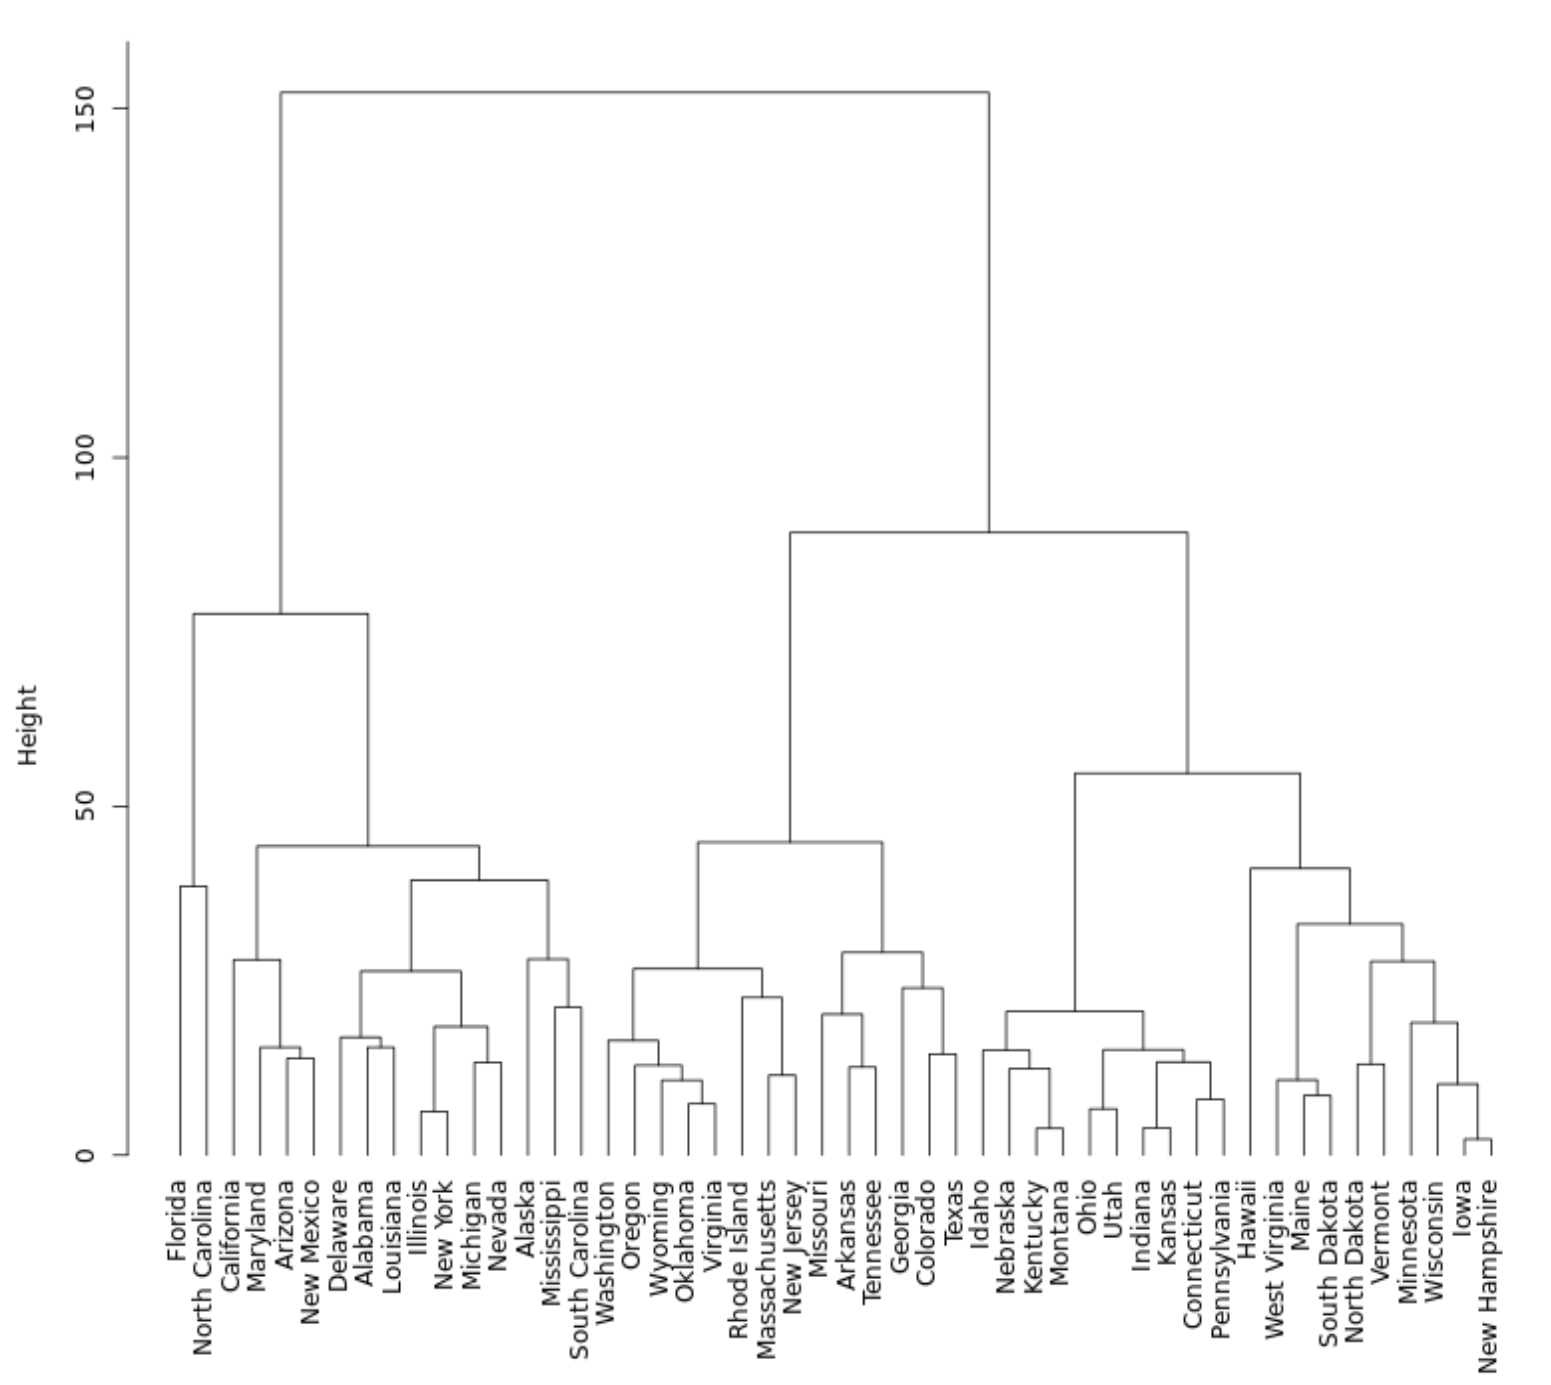
\includegraphics[width=\linewidth]{img/dendro}
	\caption{An example of dendrogram. placeholder }
	\label{fig01:dendro}
\end{figure}

To know which two clusters are connected (or respectively, how a cluster is divided into two), algorithms use a \emph{measure of a dissimilarity} between clusters.  
Hierarchical model distinguishes various kind of algorithms based on the choice of this measure. Commonly, the computation is dependent on the two factors; \emph{distance function} and \emph{linkage criterion}. 

\subsubsection{Distance functions}

\emph{Distance function} is used on objects of a dataset to express how far they are from each other in the observed domain. Supposing objects are represented as vectors $v_i \in \R_d$, variations of \emph{Minkowski distance formula} (see \ref{eq01:mink}) are the most commonly used.
This variations are \emph{Manhattan distance} ($p=1$), \emph{Euclidean distance} ($p=2$) and \emph{Chebyshev distance} ($p \to \infty$) (see \ref{tab01:mink}).

It is obvious that the choice of a distance function can influence the result of a clustering. Hence, it should be chosen with respect to the properties of a provided dataset. \citet{aggarwal2001surprising} show the qualitative behavior of different distance functions in the $k$-means algorithm.  

\begin{equation}\label{eq01:mink}
||a-b||_p = (\sum_{i=1...d}|a_i-b_i|^p)^{\frac{1}{p}}
\end{equation}

\begin{table}
	\centering
	\begin{tabular}{ll}
		\toprule
		Manhattan & $||a-b||_1 = \sum_{i=1...d}|a_i-b_i|$          \\
		Euclidean & $||a-b||_2 = \sqrt{\sum_{i=1...d}(a_i-b_i)^2}$ \\
		Chebyshev & $||a-b||_\infty = \max_{i=1\dots d}|a_i-b_i|$  \\ \bottomrule
	\end{tabular}
	\caption{Variations of Minkowski distance formula.}
	\label{tab01:mink}
\end{table}

\subsubsection{Linkage criteria}

As the reader may have already discovered, one particular problem arises. The hierarchical algorithm can not compute proximity of two clusters only using distance function as it is the function of \emph{dataset objects} Hence, we define a function of \emph{object clusters} to complete the process of measuring dissimilarity -- \emph{linkage criterion}. Supposing clusters $A$ and $B$ as sets of dataset objects and distance function $d$, wer define following \emph{linkage criteria}~\cite{yim2015hierarchical}:

\begin{description}
	\item[Single linkage] -- Also referred to as minimum method, \emph{single linkage criterion} computes distance between $A$ and $B$ as the minimum distance between any pair $(a,b) \in A\times B$ (see \ref{eq01:single_link}).
	\begin{equation}\label{eq01:single_link}
	\min\{d(a,b) : a \in A, b \in B\}
	\end{equation}
	
	The major drawback this criterion suffers is \emph{cluster chaining}. Such two clusters can be connected that they do not share any other pair of close proximity objects than the one that determined the connection. This produces long thin clusters with great distance between some objects.
	
	\item[Complete linkage] -- Also referred to as maximum method, \emph{complete linkage criterion} is similar to the single linkage criterion. But as opposed to to finding minimum, this criterion uses the maximum of object pairs in computing cluster dissimilarity (see \ref{eq01:complete_link}). 
	\begin{equation}\label{eq01:complete_link}
	\max\{d(a,b) : a \in A, b \in B\}
	\end{equation}
	
	The criterion suffers from its simplicity as well as the single linkage. But instead of naively connecting dissmimilar clusters, here simmilar clusters are not connected in some cases. Having all two clusters' objects in close proximity to each other but one object being rather far from the others, the criterion will not link the clusters as the maximum distance deteriorates the rest.
	
	\item[Centroid linkage] -- \emph{Centroid linkage criterion} tries to solve problems of criteria above by measuring the distance between the centroids of clusters. It introduces a form of an average into the computation; the think that criteria above lack.
\end{description}

\begin{figure}\centering
	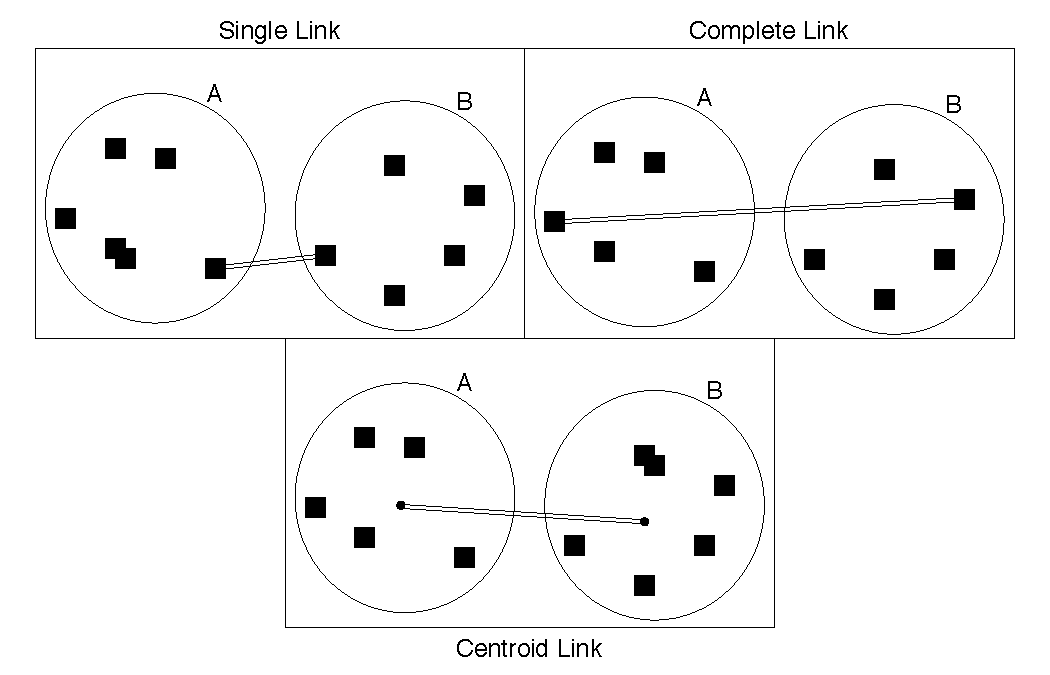
\includegraphics[width=\linewidth]{img/linkage_criteria}
	\caption{Example of linkage criteria. The double line represents the distance between clusters A and B according to respective criterion.}
	\label{fig01:link}
\end{figure}

A choice of a linkage criterion in hierarchical clustering algorithm is vital. As stated above, it can change the course of clustering in a great manner. Chosen improperly, it can have disastrous effect on the resulting solution.

\section{Mahalanobis-based clustering}

To produce more meaningful results, hierarchical clustering algorithms have branched into many variations each focusing on a specific dataset types. \emph{Ma\-ha\-la\-no\-bis-based hierarchical clustering} focuses on datasets that create clusters of ellipsoid shapes. This datasets are common products during natural measurements of cell cytometry data in bio-informatics.

\subsection{Mahalanobis distance}

The significant part of this clustering variation is the measure of cluster dissimilarity. To easily imagine the measure, suppose we have two elliptic clusters. The algorithm favors such clusters that their ellipsis are alongide rather than in prolongation of one another \cite{dagnelie1991using} (see \ref{fig01:ellipses}). 

\begin{figure}\centering
	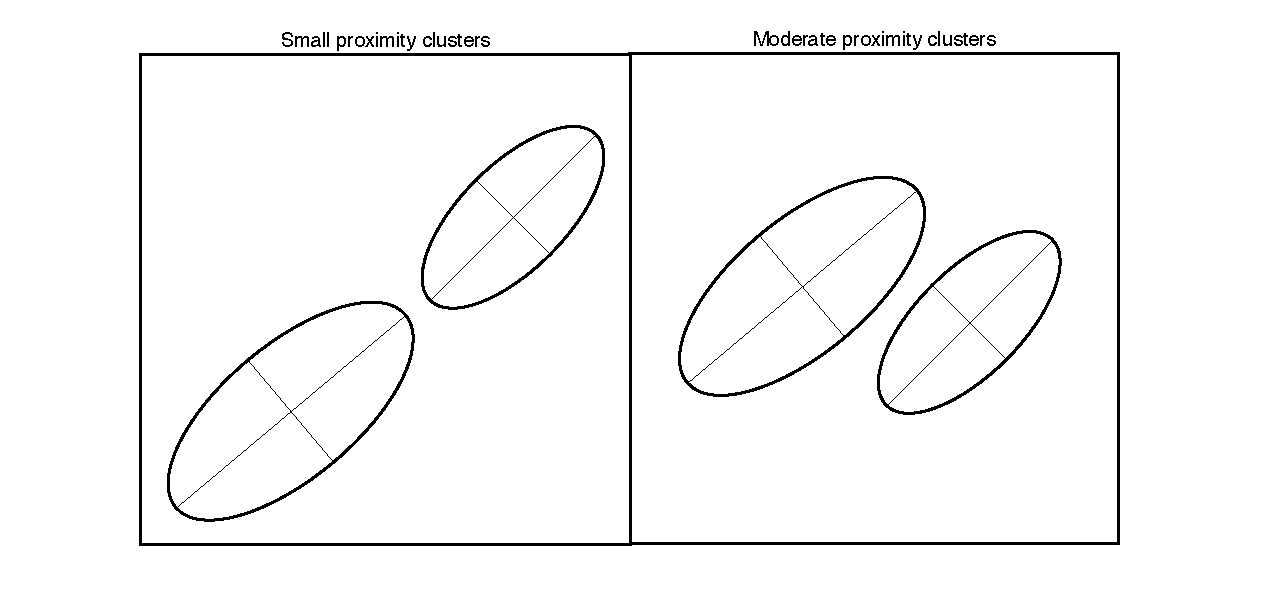
\includegraphics[width=\linewidth]{img/ellipses}
	\caption{Example of cluster dissimilarity in Mahalanobis-based hierarchical clustering.}
	\label{fig01:ellipses}
\end{figure}

\begin{defn}
	Suppose we have a cluster of $d$-dimensional points $\mathcal{C} \subset \R^d$. We define \emph{the random vector of a cluster} $\mathbf{v}$ as a $d$-element vector; $i$-th element being a discrete random variable with equal probability values $\{o_i:o\in \mathcal{C}\}$
\end{defn}

\begin{defn}
	Suppose we have a cluster of $d$-dimensional points $\mathcal{C} \subset \R^d$, the centroid $c$ of $\mathcal{C}$ and covariance matrix $\mathcal{S}$ from the random vector $\mathbf{v}$ of the cluster $\mathcal{C}$. We define \emph{Mahalanobis distance} between $u \in \R^d$ and $\mathcal{C}$ is defined by the equation \ref{eq01:maha}.
	\begin{equation}\label{eq01:maha}
	d_M(u,\mathcal{C}) = \sqrt{(u-c)^TS^{-1}(u-c)}
	\end{equation}
\end{defn}

\section{performance}
